\chapter{Anexo III - Manuales de usuario e Instalación}


En este anexo se proporcionarán los manuales de usuario e instalación de las herramientas necesarias para el desarrollo y la verificación del funcionamiento del \gls{tfm}. Además, se explicará el funcionamiento de los scripts de instalación generados, facilitando así el acceso a cualquier persona interesada en replicar los diferentes casos de uso. Los manuales de usuario detallarán los pasos necesarios para utilizar cada herramienta, incluyendo instrucciones de instalación, configuración y operación. Se proporcionarán ejemplos prácticos y se explicarán los conceptos clave relacionados con el uso de estas herramientas.\\
\\
Asimismo, se incluirá información sobre los scripts de instalación desarrollados, que permiten una instalación rápida y sencilla de las herramientas y componentes necesarios para reproducir los casos de uso del TFM. Estos scripts automatizan gran parte del proceso de instalación y configuración, lo que facilita a los usuarios la puesta en marcha de los entornos necesarios para el desarrollo y la evaluación.

%%%%%%%%%%%%%%%%%%%%%%%%%%%%%%%%%%%%%%%%%%%%%%%%%%%%%%%%%%%%%%%%%%%%%%%%%%%%%%%%%%%%%%%%%
\section{Herramienta \texttt{iproute2}}
\label{iproute2}
En el contexto del desarrollo y validación del protocolo desarrollado, la herramienta iproute2 desempeñará un papel fundamental en la configuración de las interfaces inalámbricas emuladas en el kernel, así como en la consulta del estado de estas interfaces y la verificación de la ubicación del usuario dentro de los \textit{Network namespaces}. Por tanto, se considera relevante incluir esta sección, ya que iproute2 se convertirá en una de las herramientas clave para la gestión de los \textit{Network namespaces} y la verificación de los casos de uso en la validación del protocolo desarrollado.\\
\\
iproute2 es una suite de herramientas de línea de comandos que proporciona funcionalidades avanzadas de gestión de redes en sistemas Linux. Su amplio conjunto de comandos y opciones permite realizar diversas tareas relacionadas con la configuración y administración de interfaces de red, enrutamiento, gestión de tablas de enrutamiento, configuración de políticas de tráfico y mucho más. En el contexto de este proyecto, se utilizará iproute2 para realizar acciones específicas, como configurar las interfaces inalámbricas emuladas en el kernel, verificar el estado de las interfaces y determinar en qué \textit{Network namespace} se encuentra el usuario. La inclusión de esta sección permitirá a los lectores familiarizarse con las funcionalidades básicas de iproute2 que serán relevantes para el desarrollo y verificación de los casos de uso. A lo largo de esta sección, se presentarán los comandos más utilizados y se proporcionarán ejemplos prácticos de su aplicación en el contexto del proyecto. Además, se recomendará al lector que consulte la documentación oficial de iproute2 para obtener una comprensión más completa de las capacidades y opciones avanzadas de esta herramienta.

\subsection{¿Qué es \texttt{iproute2?}}

Iproute2 es un conjunto de herramientas de utilidad para la gestión de redes en sistemas Linux. Se ha convertido en una solución ampliamente adoptada y está presente en la mayoría de las distribuciones actuales. El proyecto es mantenido por Alexey Kuznetsov y Stephen Hemminger, quienes han sido los principales desarrolladores del software. Además, iproute2 es un proyecto de código abierto en el cual contribuyen activamente cientos de personas a través de su repositorio en GitHub\footnote{\url{https://github.com/shemminger/iproute2}}.\\
\\
La versión más reciente de iproute2 es la \texttt{v6.4.0}, la cual se utilizará en el entorno de Ubuntu 18.04 para este proyecto. Este paquete de herramientas está diseñado para reemplazar a las utilidades contenidas en el paquete \textbf{net-tools}, como \texttt{ifconfig}, \texttt{route}, \texttt{netstat}, \texttt{arp}, entre otras. En la Tabla \ref{tab:ipNettools} se presenta una comparativa de las herramientas equivalentes de net-tools y las correspondientes en iproute2. La amplia adopción de iproute2 se debe a su flexibilidad y capacidad para ofrecer una amplia gama de funcionalidades para la gestión de redes en sistemas Linux. Las herramientas incluidas en iproute2 permiten configurar interfaces de red, manipular tablas de enrutamiento, establecer políticas de tráfico, supervisar el estado de las interfaces y mucho más. Su diseño modular y su enfoque en la eficiencia y el rendimiento hacen de iproute2 una opción preferida para administrar y diagnosticar redes en sistemas Linux.

\begin{table}[ht!]
    \centering
    \begin{tabular}{|c|c|}
        \hline
        \rowcolor[HTML]{C0C0C0}
        {\color[HTML]{000000} \textbf{net-tools}} & {\color[HTML]{000000} \textbf{iproute2}} \\ \hline
        \texttt{arp}                              & \texttt{ip neigh}                        \\ \hline
        \texttt{ifconfig}                         & \texttt{ip link}                         \\ \hline
        \texttt{ifconfig -a}                      & \texttt{ip addr}                         \\ \hline
        \texttt{iptunnel}                         & \texttt{ip tunnel}                       \\ \hline
        \texttt{route}                            & \texttt{ip route}                        \\ \hline
    \end{tabular}
    \caption{Herramientas de Iproute2 frente a las de net-tools}
    \label{tab:ipNettools}
\end{table}

\subsection{¿Por qué necesitamos \texttt{iproute2}?}

La justificación de utilizar el paquete de herramientas de red iproute2 para gestionar las interfaces veth, las interfaces inalámbricas emuladas del módulo del kernel \texttt{mac80211\_hwsim}, las network namespaces y la gestión con interfaces se basa en varios aspectos fundamentales:\\
\\
\begin{itemize}
    \item Funcionalidad integral: iproute2 proporciona un conjunto completo de herramientas que permiten la gestión y configuración avanzada de las interfaces de red. Esto incluye la creación, eliminación, configuración de direcciones IP, asignación de rutas, configuración de parámetros y mucho más. Al utilizar iproute2, se tiene acceso a todas estas capacidades en un solo paquete, lo que facilita la administración eficiente de las interfaces requeridas en el proyecto.

    \item Flexibilidad y compatibilidad: iproute2 es una solución ampliamente adoptada en sistemas Linux y está disponible en la mayoría de las distribuciones actuales. Al utilizar iproute2, nos aseguramos de tener una herramienta compatible y probada que nos permita gestionar las interfaces veth y las interfaces inalámbricas emuladas del módulo \texttt{mac80211\_hwsim}. Además, iproute2 es compatible con las network namespaces, lo que nos facilita la gestión y operativa de estos entornos de red aislados.

    \item Capacidad para la configuración avanzada: iproute2 proporciona opciones de configuración avanzadas que permiten un control preciso sobre las interfaces de red. Por ejemplo, podemos utilizar iproute2 para establecer políticas de tráfico, aplicar reglas de enrutamiento específicas, configurar parámetros de calidad de servicio (QoS) y más. Esto es especialmente importante en el contexto de este proyecto, donde se requiere una gestión detallada y precisa de las interfaces veth y las interfaces inalámbricas emuladas.
\end{itemize}


\subsection{Compilación e instalación de \texttt{iproute2}}

El proceso de compilación e instalación de la herramienta iproute2 es prácticamente análogo tanto en Ubuntu 20.04 como en Ubuntu 22.04, con una única diferencia que se mencionará más adelante. Antes de proceder con la compilación, es necesario realizar una configuración previa instalando los paquetes necesarios. Estos paquetes proporcionarán las dependencias requeridas para el proceso de compilación y garantizarán un entorno adecuado para la instalación de iproute2. Entre los paquetes necesarios se encuentran:

\begin{itemize}
    \item \texttt{bison}: una herramienta generadora de analizadores sintácticos de propósito general.
    \item \texttt{flex}: una herramienta para generar programas que reconocen patrones léxicos en el texto.
    \item \texttt{libmnl-dev}: una librería de espacio de usuario orientada a los desarrolladores de Netlink. Netlink es una interfaz entre el espacio de usuario y el espacio del kernel vía sockets.

    \item \texttt{libdb5.3-dev}: un paquete de desarrollo que contiene los archivos de cabecera y librerías estáticas necesarias para la base de datos de Berkley (\textit{Key/Value}).
\end{itemize}

Es importante asegurarse de tener instalado el paquete \texttt{wget} para poder descargar la herramienta iproute2. En caso de no tenerlo, se debe instalar previamente. Una vez que los paquetes necesarios estén instalados, se puede proceder con el proceso de compilación e instalación de iproute2.\\


\begin{lstlisting}[language= bash, style=Consola2, caption={Instalación de las dependencias de Iproute2},label=code:iproute2_deps]
   sudo apt-get install bison flex libmnl-dev libdb5.3-dev
\end{lstlisting}

\begin{itemize}
    \item En segundo lugar, se debe descargar el comprimido de la herramienta iproute2. Al haber varios paquetes, se descargará aquel cuya versión sea con la que se quiere trabajar. Puedes descargarlo desde el siguiente enlace: \href{https://mirrors.edge.kernel.org/pub/linux/utils/net/iproute2/}{\textbf{kernel.org}}.
\end{itemize}

\begin{lstlisting}[language= bash, style=Consola, caption={Obtención del source de Iproute2},label=code:iproute2_src]
   wget -c http://ftp.iij.ad.jp/pub/linux/kernel/linux/utils/net/iproute2/iproute2-4.15.0.tar.gz
\end{lstlisting}

\begin{itemize}
    \item En tercer lugar, se debe descomprimir el comprimido de la herramienta. A continuación, se procederá a configurar, compilar e instalar la herramienta.
\end{itemize}

\begin{lstlisting}[language= bash, style=Consola, caption={Compilación e instalación de Iproute2},label=code:iproute2_install]
   # Descomprimir y entrar al directorio
   tar -xvfz $(tar).tar.gz && cd $tar
   
   # Configurar la herramienta
   ./configura
   
   # Compilar e instalar, para añadir el nuevo binario al PATH
   sudo make
   sudo make install
\end{lstlisting}

\newpage

\subsection{Comandos útiles con \texttt{iproute2}}

A continuación, se presentan los comandos más frecuentemente utilizados con la herramienta iproute2. Estos comandos han sido ampliamente empleados a lo largo del desarrollo del proyecto y en el proceso de verificación de los distintos casos de uso. Por tanto, se considera que esta sección resultará de gran utilidad para los lectores que no estén familiarizados con esta herramienta y deseen aprender cómo utilizarla de manera efectiva.\\

\begin{lstlisting}[language= bash, style=Consola, caption={Comandos útiles con iproute2},label=code:iproute2_use]
    # Listar interfaces y visualizar las direcciones asignadas
    ip addr show
    
    # Asignar o eliminar una dirección a una interfaz
    ip addr add {IP} dev {interfaz}
    ip addr del {IP} dev {interfaz}
    
    # Activar o desactivar una interfaz
    ip link set {interfaz} up/down
    
    # Listar las rutas de red
    ip route list
    
    # Obtener la ruta para una dirección IP específica
    ip route get {IP}
    
    # Listar los Network namespaces con sus nombres asignados
    ip netns list
    
    # Si lees esto, te debo un besito :)
\end{lstlisting}
\vspace{0.5cm}
Estos comandos proporcionan funcionalidades clave para la administración y configuración de interfaces de red, rutas de red y namespaces de red. Al utilizarlos de manera adecuada, los administradores de redes pueden llevar a cabo tareas importantes, como la asignación de direcciones IP, la habilitación o deshabilitación de interfaces, el enrutamiento de paquetes y la gestión de entornos de red aislados. Por lo tanto, comprender y dominar estos comandos resulta fundamental para cualquier profesional o entusiasta de las redes que desee tener un control preciso sobre su infraestructura de red.
\newpage
%%%%%%%%%%%%%%%%%%%%%%%%%%%%%%%%%%%%%%%%%%%%%%%%%%%%%%%%%%%%%%%%%%%%%%%%%%%%%%%%%%%%%%%%%%%%%%%%%%

\section{Herramienta \texttt{tcpdump}}
\label{tcpdump}

La inclusión de esta sección se motiva por proporcionar un punto de referencia para aquellos usuarios que no están familiarizados con tcpdump. A lo largo de todas las secciones del proyecto, se utilizará esta herramienta para verificar el correcto funcionamiento de los casos de uso. El objetivo de esta sección es ofrecer una guía práctica sobre cómo utilizar tcpdump, especialmente dirigida a aquellos usuarios que no tienen experiencia previa con la herramienta. Se proporcionarán instrucciones detalladas sobre cómo instalar y ejecutar tcpdump, así como ejemplos de comandos comunes para capturar y analizar el tráfico de red.\\
\\
Al comprender cómo utilizar tcpdump, los usuarios podrán verificar de manera efectiva si los casos de uso implementados en el proyecto están funcionando según lo esperado. Esta herramienta les permitirá examinar el tráfico de red en tiempo real y obtener información relevante para la evaluación y solución de problemas.

\subsection{¿Qué es \texttt{tcpdump}?}

Tcpdump es un analizador de tráfico diseñado para inspeccionar los paquetes entrantes y salientes de una interfaz. La peculiaridad de esta herramienta es que funciona mediante línea de comandos y tiene soporte en la mayoría de los sistemas UNIX\footnote{Unix es un sistema operativo desarrollado en 1969 por un grupo de empleados de los laboratorios Bell}, como Linux, macOS y OpenWrt. La herramienta está escrita en lenguaje C, lo que le confiere un alto rendimiento, y utiliza libpcap\footnote{\url{https://github.com/the-tcpdump-group/libpcap}} para la captura de paquetes.\\
\\
Fue desarrollada en 1988 por trabajadores de los laboratorios de Berkeley. En la actualidad, cuenta con una gran comunidad de desarrolladores respaldándola en su repositorio oficial\footnote{\url{https://github.com/the-tcpdump-group/tcpdump}}, donde se lanzan periódicamente nuevas actualizaciones (última versión \texttt{v4.99.4}).

\subsection{¿Por qué necesitamos \texttt{tcpdump}?}

En la actualidad, es común desarrollar en entornos distribuidos, utilizando contenedores o máquinas virtuales para delimitar el entorno de desarrollo. Por esta razón, se trabaja de forma remota, conectándose a la máquina o contenedor mediante el protocolo SSH\footnote{\url{https://www.ssh.com/ssh/}}.\\
\\
Esto conlleva numerosas ventajas, pero también puede presentar complicaciones. Por ejemplo, si alguien no sabe cómo configurar un \textit{X Server} para ejecutar aplicaciones gráficas de forma remota, no podría utilizar herramientas como Wireshark. En este sentido, tcpdump resulta especialmente útil, ya que no requiere ninguna configuración adicional para ejecutarse de forma remota. Además, su rápido inicio, en comparación con otros ``sniffers" como Wireshark, ha convertido a tcpdump en una herramienta fundamental para verificar casos de uso.

\subsection{Instalación de \texttt{tcpdump}}

Como se mencionó anteriormente, tcpdump cuenta con un amplio soporte en sistemas UNIX, por lo que suele estar preinstalado en la mayoría de las distribuciones Linux. Sin embargo, en caso de no tenerlo instalado, es posible instalarlo fácilmente siguiendo los pasos que se muestran a continuación (Ver bloque \ref{code:tcpdump}). Estos comandos actualizarán los repositorios de paquetes y descargarán e instalarán tcpdump en el sistema. Una vez completada la instalación, tcpdump estará listo para su uso.

\begin{lstlisting}[language= bash, style=Consola2, caption={Instalación del paquete Tcpdump},label=code:tcpdump]
    sudo apt install -y tcpdump
\end{lstlisting}

\subsection{Comandos útiles con \texttt{tcpdump}}


A continuación, se presentan algunos comandos comunes que se han utilizado durante el proceso de verificación de los casos de uso con la herramienta tcpdump. Estos comandos han sido seleccionados debido a su relevancia y utilidad, y se considera que pueden ser de gran ayuda para aquellos lectores que no estén familiarizados con esta herramienta. No obstante, se recomienda encarecidamente que el lector consulte la página de manual de tcpdump\footnote{\url{https://linux.die.net/man/8/tcpdump}} para obtener información más detallada sobre el uso básico de tcpdump y explorar todas sus capacidades. Estos son solo algunos ejemplos de los comandos más utilizados con tcpdump. Como se mencionó anteriormente, se recomienda encarecidamente al lector que consulte la página de manual de tcpdump para obtener una comprensión más completa de sus capacidades y explorar otros filtros y opciones disponibles.

\begin{lstlisting}[language= bash, style=Consola2, caption={Comandos útiles con Tcpdump},label=code:tcpdump_use]
    # Indicar sobre que Interfaz se quiere sniffear
    tcpdump -i {Interfaz}
    
    # Podemos almacenar la traza a un archivo para su posterior análisis
    tcpdump -w fichero.pcap -i {Interfaz}
    
    # También podemos ver una traza desde un archivo
    tcpdump -r fichero.pcap
    
    # Podemos filtrar por  puerto
    tcpdump -i {Interfaz} port {Puerto}
    
    # Podemos filtrar por  dirección IP destino/origen
    tcpdump -i {Interfaz} dst/src {IP}
    
    # Podemos filtrar por protocolo
    tcpdump -i {Interfaz} {protocolo}
    
    # Listar interfaces disponibles para escuchar de ellas 
    tcpdump -D
    
     # Limitar el número de paquetes a sniffear
    tcpdump -i {Interfaz} -c {Número de paquetes}
\end{lstlisting}
\vspace{1cm}
\begin{figure}[ht]
    \centering
    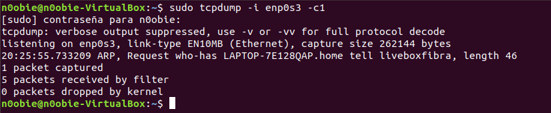
\includegraphics[width=\textwidth]{archivos/img/anexos/tcpdump_cli_edited.png}
    \caption{Interfaz de tipo CLI de Tcpdump}
    \label{tcpdumpCli}
\end{figure}

%%%%%%%%%%%%%%%%%%%%%%%%%%%%%%%%%%%%%%%%%%%%%%%%%%%%%%%%%%%%%%%%%%%%%%%%%%%%%%%%%%%%%%%%%%%%%%%%%%
\newpage
\section{Herramienta Mininet}
\label{sec:ToolsMininet}
La motivación de añadir esta sección es la de poder indicar al lector como se ha instalado la herramienta de Mininet en las distintas máquinas descritas en el pliego de condiciones (Anexo \ref{ch:anexoPliegoCondiciones}). Todo el proceso de instalación se ha llevado acabo en una máquina Linux, con las especificaciones indicadas en la siguiente tabla (Tabla \ref{tab:ToolsMininet}).

\begin{table}[ht!]
    \centering
    \resizebox{0.6\columnwidth}{!}{%
        \begin{tabular}{|c|c|c|c|}
            \hline
            \rowcolor[HTML]{EFEFEF}
            \textbf{Distribución Linux} & \textbf{Cores} & \textbf{Memoria} & \textbf{Disco} \\ \hline
            Ubuntu 22.04 LTS            & 2              & 4096 MiB         & 40 GiB         \\ \hline
        \end{tabular}%
    }
    \caption{Especificaciones máquina de instalación Mininet}
    \label{tab:ToolsMininet}
\end{table}

Para la instalación necesitaremos de conectividad a Internet y de la herramienta \texttt{git} para clonar el repositorio de \texttt{Mininet}. En caso de no tener la herramienta de \texttt{git}, podremos instalarla ejecutando el comando del bloque de código \ref{code:git_install}.

\begin{lstlisting}[language= bash, style=Consola2, caption={Instalación de la herramienta git},label=code:git_install]
    # El parametro -y se indica para confirmar la instalación de la herramienta
    sudo apt install -y git 
\end{lstlisting}
\vspace{1cm}

Una vez disponemos de la herramienta \texttt{git} para clonar el repositorio de \texttt{Mininet}, vamos a clonarlo, y lanzar el script de instalación que incorpora junto al source para instalar la herramineta. A continuación, en el bloque de código \ref{code:Mininet_install} se indica los comandos ejecutados para instalar la herrmaienta de \texttt{Mininet}.


\begin{lstlisting}[language= bash, style=Consola2, caption={Instalación de la herramienta Mininet},label=code:Mininet_install]
    # Clonamos el repositorio de Mininet
    git clone https://github.com/davidcawork/mininet.git

    # Accedemos al directorio
    cd mininet

    # Lanzamos el script de instalación (Openflow 1.3 - Ryu - Wireshark dissector)
    sudo util/install.sh -3fmnyv
\end{lstlisting}
\vspace{1cm}

%%%%%%%%%%%%%%%%%%%%%%%%%%%%%%%%%%%%%%%%%%%%%%%%%%%%%%%%%%%%%%%%%%%%%%%%%%%%%%%%%%%%%%%%%%%%%%%%%%
\newpage
\section{Herramienta Mininet-WiFi}
\label{sec:ToolsMininetwifi}
La motivación de añadir esta sección es la de poder indicar al lector como se ha instalado la herramienta de Mininet en las distintas máquinas descritas en el pliego de condiciones (Anexo \ref{ch:anexoPliegoCondiciones}). Todo el proceso de instalación se ha llevado acabo en una máquina Linux, con las especificaciones indicadas en la siguiente tabla (Tabla \ref{tab:ToolsMininetWifi}).

\begin{table}[ht!]
    \centering
    \resizebox{0.6\columnwidth}{!}{%
        \begin{tabular}{|c|c|c|c|}
            \hline
            \rowcolor[HTML]{EFEFEF}
            \textbf{Distribución Linux} & \textbf{Cores} & \textbf{Memoria} & \textbf{Disco} \\ \hline
            Ubuntu 22.04 LTS            & 2              & 4096 MiB         & 40 GiB         \\ \hline
        \end{tabular}%
    }
    \caption{Especificaciones máquina de instalación Mininet-WiFi}
    \label{tab:ToolsMininetWifi}
\end{table}

Para la instalación necesitaremos de conectividad a Internet y de la herramienta \texttt{git} para clonar el repositorio de \texttt{Mininet-WiFi}. En caso de no tener la herramienta de \texttt{git}, podremos instalarla ejecutando el comando del bloque de código \ref{code:git_install}. Una vez disponemos de la herramienta \texttt{git} para clonar el repositorio de \texttt{Mininet-WiFi}, vamos a clonarlo, y lanzar el script de instalación que incorpora junto al source para instalar la herramineta. A continuación, en el bloque de código \ref{code:Mininet_wifi_install} se indica los comandos ejecutados para instalar la herrmaienta de \texttt{Mininet-WiFi}.


\begin{lstlisting}[language= bash, style=Consola2, caption={Instalación de la herramienta Mininet-WiFi},label=code:Mininet_wifi_install]
    # Clonamos el repositorio de Mininet
    git clone https://github.com/davidcawork/mininet.git

    # Accedemos al directorio
    cd mininet-wifi

    # Lanzamos el script de instalación (Openflow 1.3 - Ryu - Wireshark dissector)
    sudo ./util/install.sh -3Wlfnv

    # Para esta versión que instala vagrant de ubuntu el kernel que trae
    # no lleva el modulo mac80211_hwsim por tanto hay que añadirlo, si tu version tiene
    # compilado el modulo del kernel mac80211_hwsim, no hará falta hacer esto
    sudo apt-get install -y linux-modules-extra-5.15.0-69-generic
\end{lstlisting}
\vspace{1cm}

%%%%%%%%%%%%%%%%%%%%%%%%%%%%%%%%%%%%%%%%%%%%%%%%%%%%%%%5
\newpage
\section{Herramienta Ryu}
\label{sec:ToolsRyu}
La motivación de añadir esta sección es la de poder indicar al lector como se ha instalado la herramienta de Ryu en las distintas máquinas descritas en el pliego de condiciones (Anexo \ref{ch:anexoPliegoCondiciones}). Todo el proceso de instalación se ha llevado acabo en una máquina Linux, con las especificaciones indicadas en la siguiente tabla (Tabla \ref{tab:ToolsRyu}).

\begin{table}[ht!]
    \centering
    \resizebox{0.6\columnwidth}{!}{%
        \begin{tabular}{|c|c|c|c|}
            \hline
            \rowcolor[HTML]{EFEFEF}
            \textbf{Distribución Linux} & \textbf{Cores} & \textbf{Memoria} & \textbf{Disco} \\ \hline
            Ubuntu 22.04 LTS            & 2              & 4096 MiB         & 40 GiB         \\ \hline
        \end{tabular}%
    }
    \caption{Especificaciones máquina de instalación de Ryu}
    \label{tab:ToolsRyu}
\end{table}

Para la instalación necesitaremos de conectividad a Internet y de la herramienta \texttt{git} para clonar el repositorio de \texttt{Ryu}. En caso de no tener la herramienta de \texttt{git}, podremos instalarla ejecutando el comando del bloque de código \ref{code:git_install}. Una vez disponemos de la herramienta \texttt{git} para clonar el repositorio de \texttt{Ryu}, vamos a clonarlo, y lanzar el script de instalación que incorpora junto al source para instalar la herramineta. A continuación, en el bloque de código \ref{code:Ryu} se indica los comandos ejecutados para instalar la herrmaienta de \texttt{Ryu}.


\begin{lstlisting}[language= bash, style=Consola2, caption={Instalación de la herramienta Ryu},label=code:Ryu]
    #!/bin/bash

    echo "[+] Installing Ryu..."
    
    INSTALL='sudo DEBIAN_FRONTEND=noninteractive apt-get -y -q install'
    BUILD_DIR=${HOME}
    
    # Update
    sudo apt-get update
    
    # Install Ryu dependencies
    $INSTALL autoconf automake git g++ libtool python3 make gcc python3-pip python3-dev libffi-dev libssl-dev libxml2-dev libxslt1-dev zlib1g-dev
    
    # Fetch RYU
    cd $BUILD_DIR/
    git clone https://github.com/davidcawork/ryu.git ryu
    cd ryu
    
    # Install ryu
    sudo pip3 install -r tools/pip-requires -r tools/optional-requires \
        -r tools/test-requires
    sudo python3 setup.py install
\end{lstlisting}
\vspace{1cm}


%%%%%%%%%%%%%%%%%%%%%%%%%%%%%%%%%%%%%%%%%%%%%%%%%%%%%%%5
\newpage
\section{Herramienta ONOS}
\label{sec:ToolsOnos}
La motivación de añadir esta sección es la de poder indicar al lector como se ha instalado la herramienta de ONOS en las distintas máquinas descritas en el pliego de condiciones (Anexo \ref{ch:anexoPliegoCondiciones}). Todo el proceso de instalación se ha llevado acabo en una máquina Linux, con las especificaciones indicadas en la siguiente tabla (Tabla \ref{tab:ToolsOnos}).

\begin{table}[ht!]
    \centering
    \resizebox{0.6\columnwidth}{!}{%
        \begin{tabular}{|c|c|c|c|}
            \hline
            \rowcolor[HTML]{EFEFEF}
            \textbf{Distribución Linux} & \textbf{Cores} & \textbf{Memoria} & \textbf{Disco} \\ \hline
            Ubuntu 22.04 LTS            & 2              & 4096 MiB         & 40 GiB         \\ \hline
        \end{tabular}%
    }
    \caption{Especificaciones máquina de instalación de ONOS}
    \label{tab:ToolsOnos}
\end{table}

Para la instalación necesitaremos de conectividad a Internet y de la herramienta \texttt{git} para clonar el repositorio de \texttt{ONOS} y las herramientas asociadas. En caso de no tener la herramienta de \texttt{git}, podremos instalarla ejecutando el comando del bloque de código \ref{code:git_install}. Una vez disponemos de la herramienta \texttt{git} para clonar el repositorio de \texttt{ONOS}, vamos a clonarlo, y lanzar el script de instalación que incorpora junto al source para instalar la herramineta. A continuación, en el bloque de código \ref{code:ONOS} se indica los comandos ejecutados para instalar la herrmaienta de \texttt{ONOS}.


\begin{lstlisting}[language= bash, style=Consola2, caption={Instalación de la herramienta ONOS},label=code:ONOS]
    #!/bin/bash

    sudo apt update -y
    sudo apt install -y git g++ unzip zip openjdk-11-jdk bzip2
    
    wget -c  https://github.com/bazelbuild/bazel/releases/download/6.0.0-pre.20220421.3/bazel-6.0.0-pre.20220421.3-installer-linux-x86_64.sh
    chmod +x bazel-6.0.0-pre.20220421.3-installer-linux-x86_64.sh
    ./bazel-6.0.0-pre.20220421.3-installer-linux-x86_64.sh --user 
    export PATH=$PATH:$HOME/bin
    
    
    git clone https://gerrit.onosproject.org/onos -b onos-2.5
    echo "#ONOS" | tee -a ~/.bashrc
    echo ". ~/onos/tools/dev/bash_profile" | tee -a ~/.bashrc
    source .bashrc
    cd onos && bazel build onos 
\end{lstlisting}
\vspace{1cm}

%%%%%%%%%%%%%%%%%%%%%%%%%%%%%%%%%%%%%%%%%%%%%%%%%%%%%%%%%%%%%%%%%%%%%%%%%%%%%%%%%%%%%%%%%%%%%%%%%%